\documentclass[conference]{IEEEtran}
\usepackage[T1]{fontenc}
\usepackage[utf8]{inputenc}
\usepackage{graphicx}
\usepackage{booktabs}
\usepackage{amsmath,amssymb}
\usepackage{algorithm}
\usepackage{algorithmic}
\usepackage{textcomp}
\usepackage{multirow}
\graphicspath{{paper_assets/diagrams/}{paper_assets/figures/}}

\begin{document}

\title{EcoMind-AI: An Offline, Data-Quality-First Platform for Trustworthy Energy Forecasting with Explainable Models and Confidence Gating}

\author{\IEEEauthorblockN{EcoMind-AI Research Team}
\IEEEauthorblockA{Metrics reproduced from the live EcoMind-AI deployment}}

\maketitle

\begin{abstract}
Reliable machine learning for building energy analytics depends as much on data quality and deployment discipline as on model choice, yet most pipelines treat these as afterthoughts and run as opaque cloud services. We present EcoMind-AI, an offline, self-contained energy-intelligence platform that couples a data-quality (DQ) engine, temporal model benchmarking, SHAP-based explainability, and a weighted confidence gate into a single auditable 17-stage workflow. On an hourly energy dataset of 3{,}600 rows (43{,}200 cells, 5 assets, 30 days), the platform evaluates 8 rules across 5 DQ dimensions; every rule passes, with per-rule scores of 96.7--100 on a 0--100 scale. A chronological 70/30 benchmark of four regressors ranks gradient boosting first among legitimate learners ($R^2=0.9175$, RMSE 1.3517) and exposes a target-leakage artifact in ridge regression ($R^2=1.0000$) caused by pre-split feature derivation, which we document as a case study rather than a result. Explanations are produced with SHAP and scored by a two-half-sample Spearman stability index. A weighted trust gate ($0.40/0.25/0.20/0.15$) fuses prediction confidence, DQ score, model relevance, and explanation stability into a trust score of 94.5/100 (high trust). Finally, a raw-versus-processed comparison reports $\Delta R^2 = 0.000$ on this already-clean dataset, an honest null result confirming that cleaning benefit is data-dependent. All artifacts, numbers, and figures are generated from the deployed system and require no network access at run time.
\end{abstract}

\begin{IEEEkeywords}
data quality, energy forecasting, gradient boosting, SHAP, trustworthy machine learning, explainable AI, MLOps
\end{IEEEkeywords}

\section{Introduction}

Building energy datasets are noisy, irregularly sampled, and routinely consumed by forecasting pipelines without systematic validation~\cite{amasyali:2018, wang:1996}. The consequences are well known: silent nulls and sensor stalls degrade accuracy, feature engineering performed before train/test splitting induces target leakage, and deployed models are shipped without calibrated evidence that their explanations are stable. Meanwhile, operational platforms for such pipelines are typically hosted services, which conflicts with the data-governance needs of facilities that cannot export meter data.

EcoMind-AI is built around a data-quality-first thesis: \emph{audit the data before trusting the model}, and carry an auditable trust signal all the way to the executive report. The platform is offline and self-contained---dataset files never leave the host machine---and exposes the entire lifecycle as an explicit 17-stage workflow streamed to the browser over server-sent events (SSE).

The contributions of this paper are:
\begin{enumerate}
\item An offline, end-to-end energy-intelligence platform implementing a 17-stage auditable workflow (library $\rightarrow$ import $\rightarrow$ preview $\rightarrow$ schema $\rightarrow$ data quality $\rightarrow$ transformation $\rightarrow$ feature engineering $\rightarrow$ prediction $\rightarrow$ confidence gate $\rightarrow$ raw-vs-processed $\rightarrow$ SHAP $\rightarrow$ anomaly $\rightarrow$ benchmarking $\rightarrow$ recommendation $\rightarrow$ executive $\rightarrow$ report $\rightarrow$ registry) on a FastAPI + SQLite + React stack (Section~\ref{sec:arch}).
\item A DQ engine of 8 rules over 5 dimensions with explicit per-rule scoring formulas, dimension aggregation, and integration of the DQ score as a weighted input to a deployment trust gate (Section~\ref{sec:dq}).
\item A leakage-aware benchmarking protocol: a chronological 70/30 holdout over four regressors, in which the platform surfaces a real target-leakage case ($y_t = \text{diff\_1h} + \text{lag\_1h}$) that drives ridge regression to $R^2=1.0000$ (Section~\ref{sec:bench}).
\item A confidence gate that fuses prediction confidence, DQ score, model relevance, and explanation stability into a single trust score, together with an honest raw-vs-processed null result ($\Delta R^2 = 0.0$) demonstrating that cleaning benefit is conditional on input quality (Section~\ref{sec:trust}, \ref{sec:rawproc}).
\end{enumerate}

\section{Related Work}\label{sec:related}

\paragraph{Data quality frameworks.}
Wang and Strong's foundational taxonomy~\cite{wang:1996} separated accuracy from broader fitness-for-use dimensions (completeness, consistency, timeliness, relevance), a structure our rule set instantiates directly for time series. Where prior work proposes descriptive quality models, EcoMind-AI operationalizes them as executable rules with pass/fail thresholds wired into a deployment gate, so that quality assessment is a runtime control rather than a report.

\paragraph{Building energy forecasting.}
The data-driven building energy prediction literature is dominated by tree ensembles and gradient boosting on engineered temporal features~\cite{amasyali:2018, chen:2016, breiman:2001}, and large public meter corpora such as BDG2~\cite{miller:2020, miller:2020gep} provide evaluation substrate. Our benchmark protocol follows this recipe (scikit-learn~\cite{pedregosa:2011} regressors on lag/rolling features) but adds a quality gate and explanation-stability scoring that these studies typically omit.

\paragraph{Temporal validation and leakage.}
Bergmeir and Benítez~\cite{bergmeir:2012} argue that out-of-sample evaluation for time series can be valid under mild dependence assumptions, yet the more common failure we observe is not shuffling but \emph{pre-split feature derivation}: computing target-derived lags and differences before the split leaks the target into the feature matrix. Our ridge $R^2=1.0000$ case is a concrete instance of this failure mode and motivates a split-then-derive discipline, consistent with forecasting practice~\cite{hyndman:2021}.

\paragraph{Explainability and trust.}
SHAP~\cite{lundberg:2017} provides additive attributions for tree models; we additionally require that explanation \emph{rankings} be reproducible across resamples, measured by a Spearman stability index. Confidence calibration and trust research~\cite{guo:2017} motivates gating on reliability signals; our gate is a weighted audit composite of four evidence factors rather than a probabilistic calibrator, and we report it as such.

\paragraph{Positioning.}
EcoMind-AI differs from cloud AutoML pipelines in three ways: quality assessment precedes modeling and feeds the gate; every stage is explicit, persisted, and streamed; and the system reports null and negative results (raw-vs-processed $\Delta R^2=0$) as first-class outcomes instead of suppressing them.

\section{System Architecture}\label{sec:arch}

\begin{figure*}[!t]
\centering
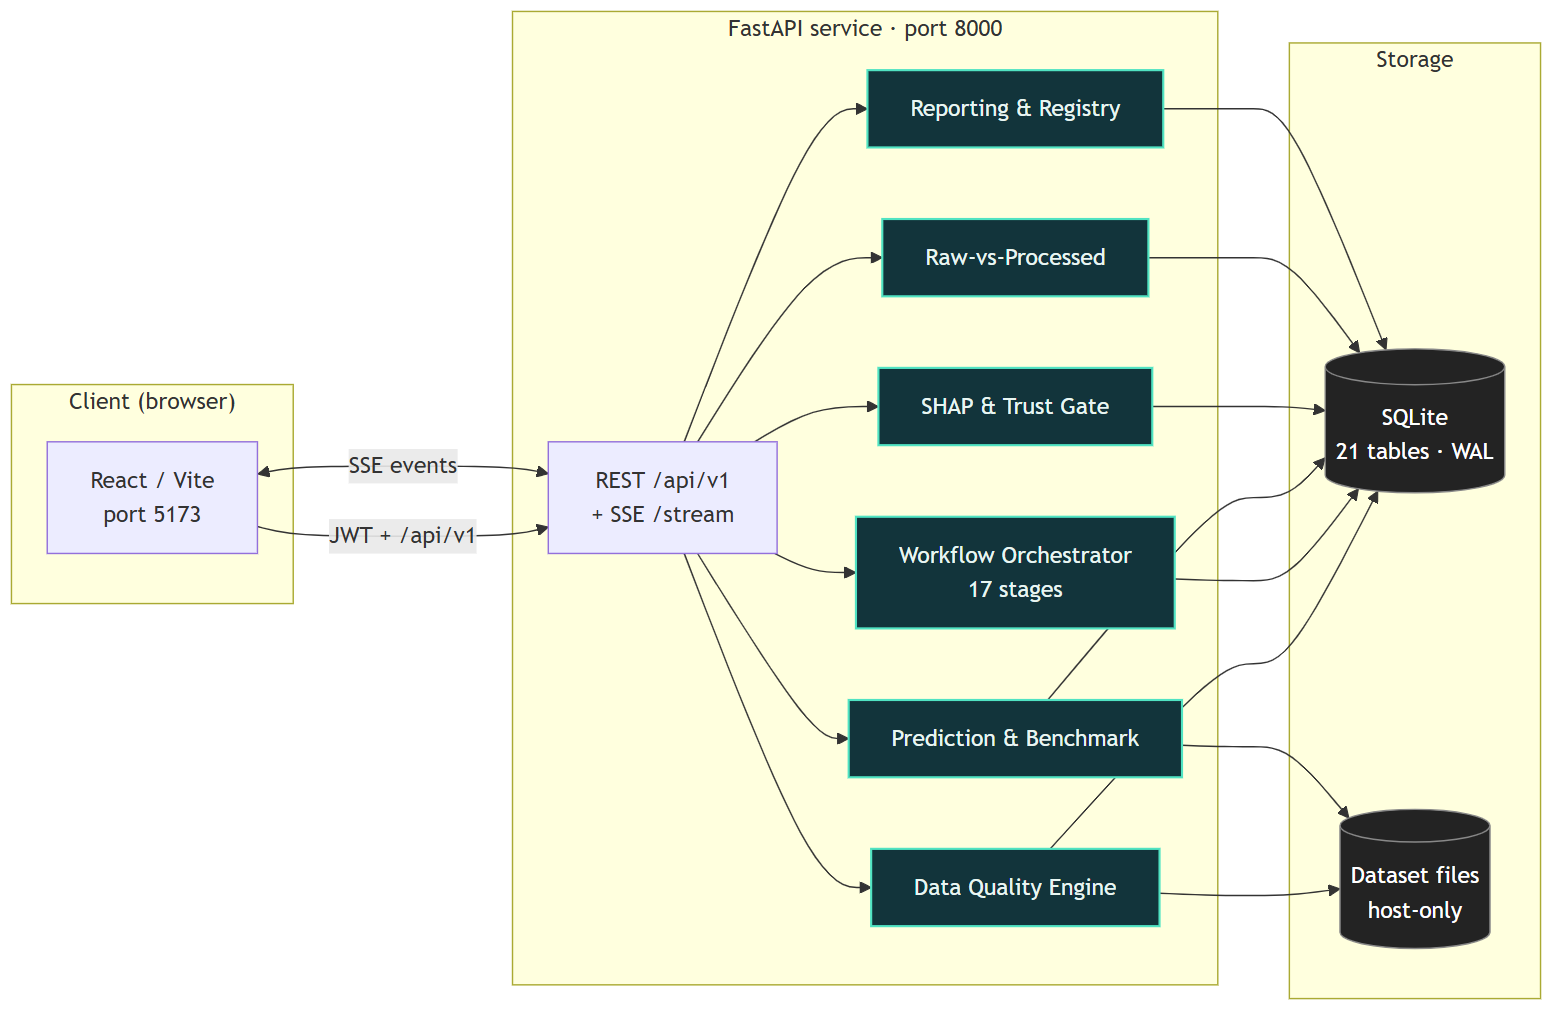
\includegraphics[width=\textwidth]{system-architecture}
\caption{EcoMind-AI system architecture. The React/Vite client talks to a FastAPI service over a JWT-authenticated \texttt{/api/v1} REST surface plus a \texttt{/stream} SSE channel for live workflow events. Domain services cover datasets and data quality, workflow orchestration, prediction and benchmarking, SHAP explanation, raw-vs-processed comparison, trust gating, reporting, and registry. State persists in a 21-table SQLite database (WAL). The deployment boundary is offline: dataset files never leave the host.}
\label{fig:arch}
\end{figure*}

The platform (Fig.~\ref{fig:arch}) is a three-tier system. A React/Vite client (port 5173) proxies \texttt{/api/v1} and \texttt{/stream} to a FastAPI backend (port 8000). Authentication is JWT bearer-based with a default local account; all API responses follow a \texttt{\{data\} | \{error\}\}} envelope. Domain logic is organized into 18 route modules (55 endpoints) covering datasets, schema, data quality, transformations, features, prediction, explanation, anomalies, benchmarks, recommendations, reports, workflows, trust, comparison, and registry.

\subsection{Workflow engine}
The core abstraction is a 17-stage workflow run persisted in SQLite. Each stage executes synchronously via \texttt{POST /workflows/\{run\_id\}/stages/\{key\}/exec} or \texttt{/advance}; runs transition \texttt{running} $\rightarrow$ \texttt{completed} only after all 17 stage keys have executed, and to \texttt{failed} if any stage raises. Stage progress is broadcast over SSE (\texttt{stage.enter}, \texttt{stage.progress}, \texttt{stage.complete}, \texttt{quality.score}, \texttt{model.metrics}, \texttt{run.done}, \ldots), which the client renders as a milestone rail (Intake, Understand, Rebuild, Model, Prove, Decide). Because execution is explicit and persisted, every reported number is traceable to a stored run.

\subsection{Data model}
Twenty-one tables model datasets, workflow runs, DQ results, models, benchmarks, registry entries, raw-vs-processed comparisons, comparison charts, predictions, anomalies, recommendations, and reports. Fig.~\ref{fig:er} shows the core entities: users own datasets and runs; datasets fan out to DQ results, models, and benchmarks; runs fan out to models, comparisons, and reports; each model maps to at most one registry entry.

\begin{figure}[!t]
\centering
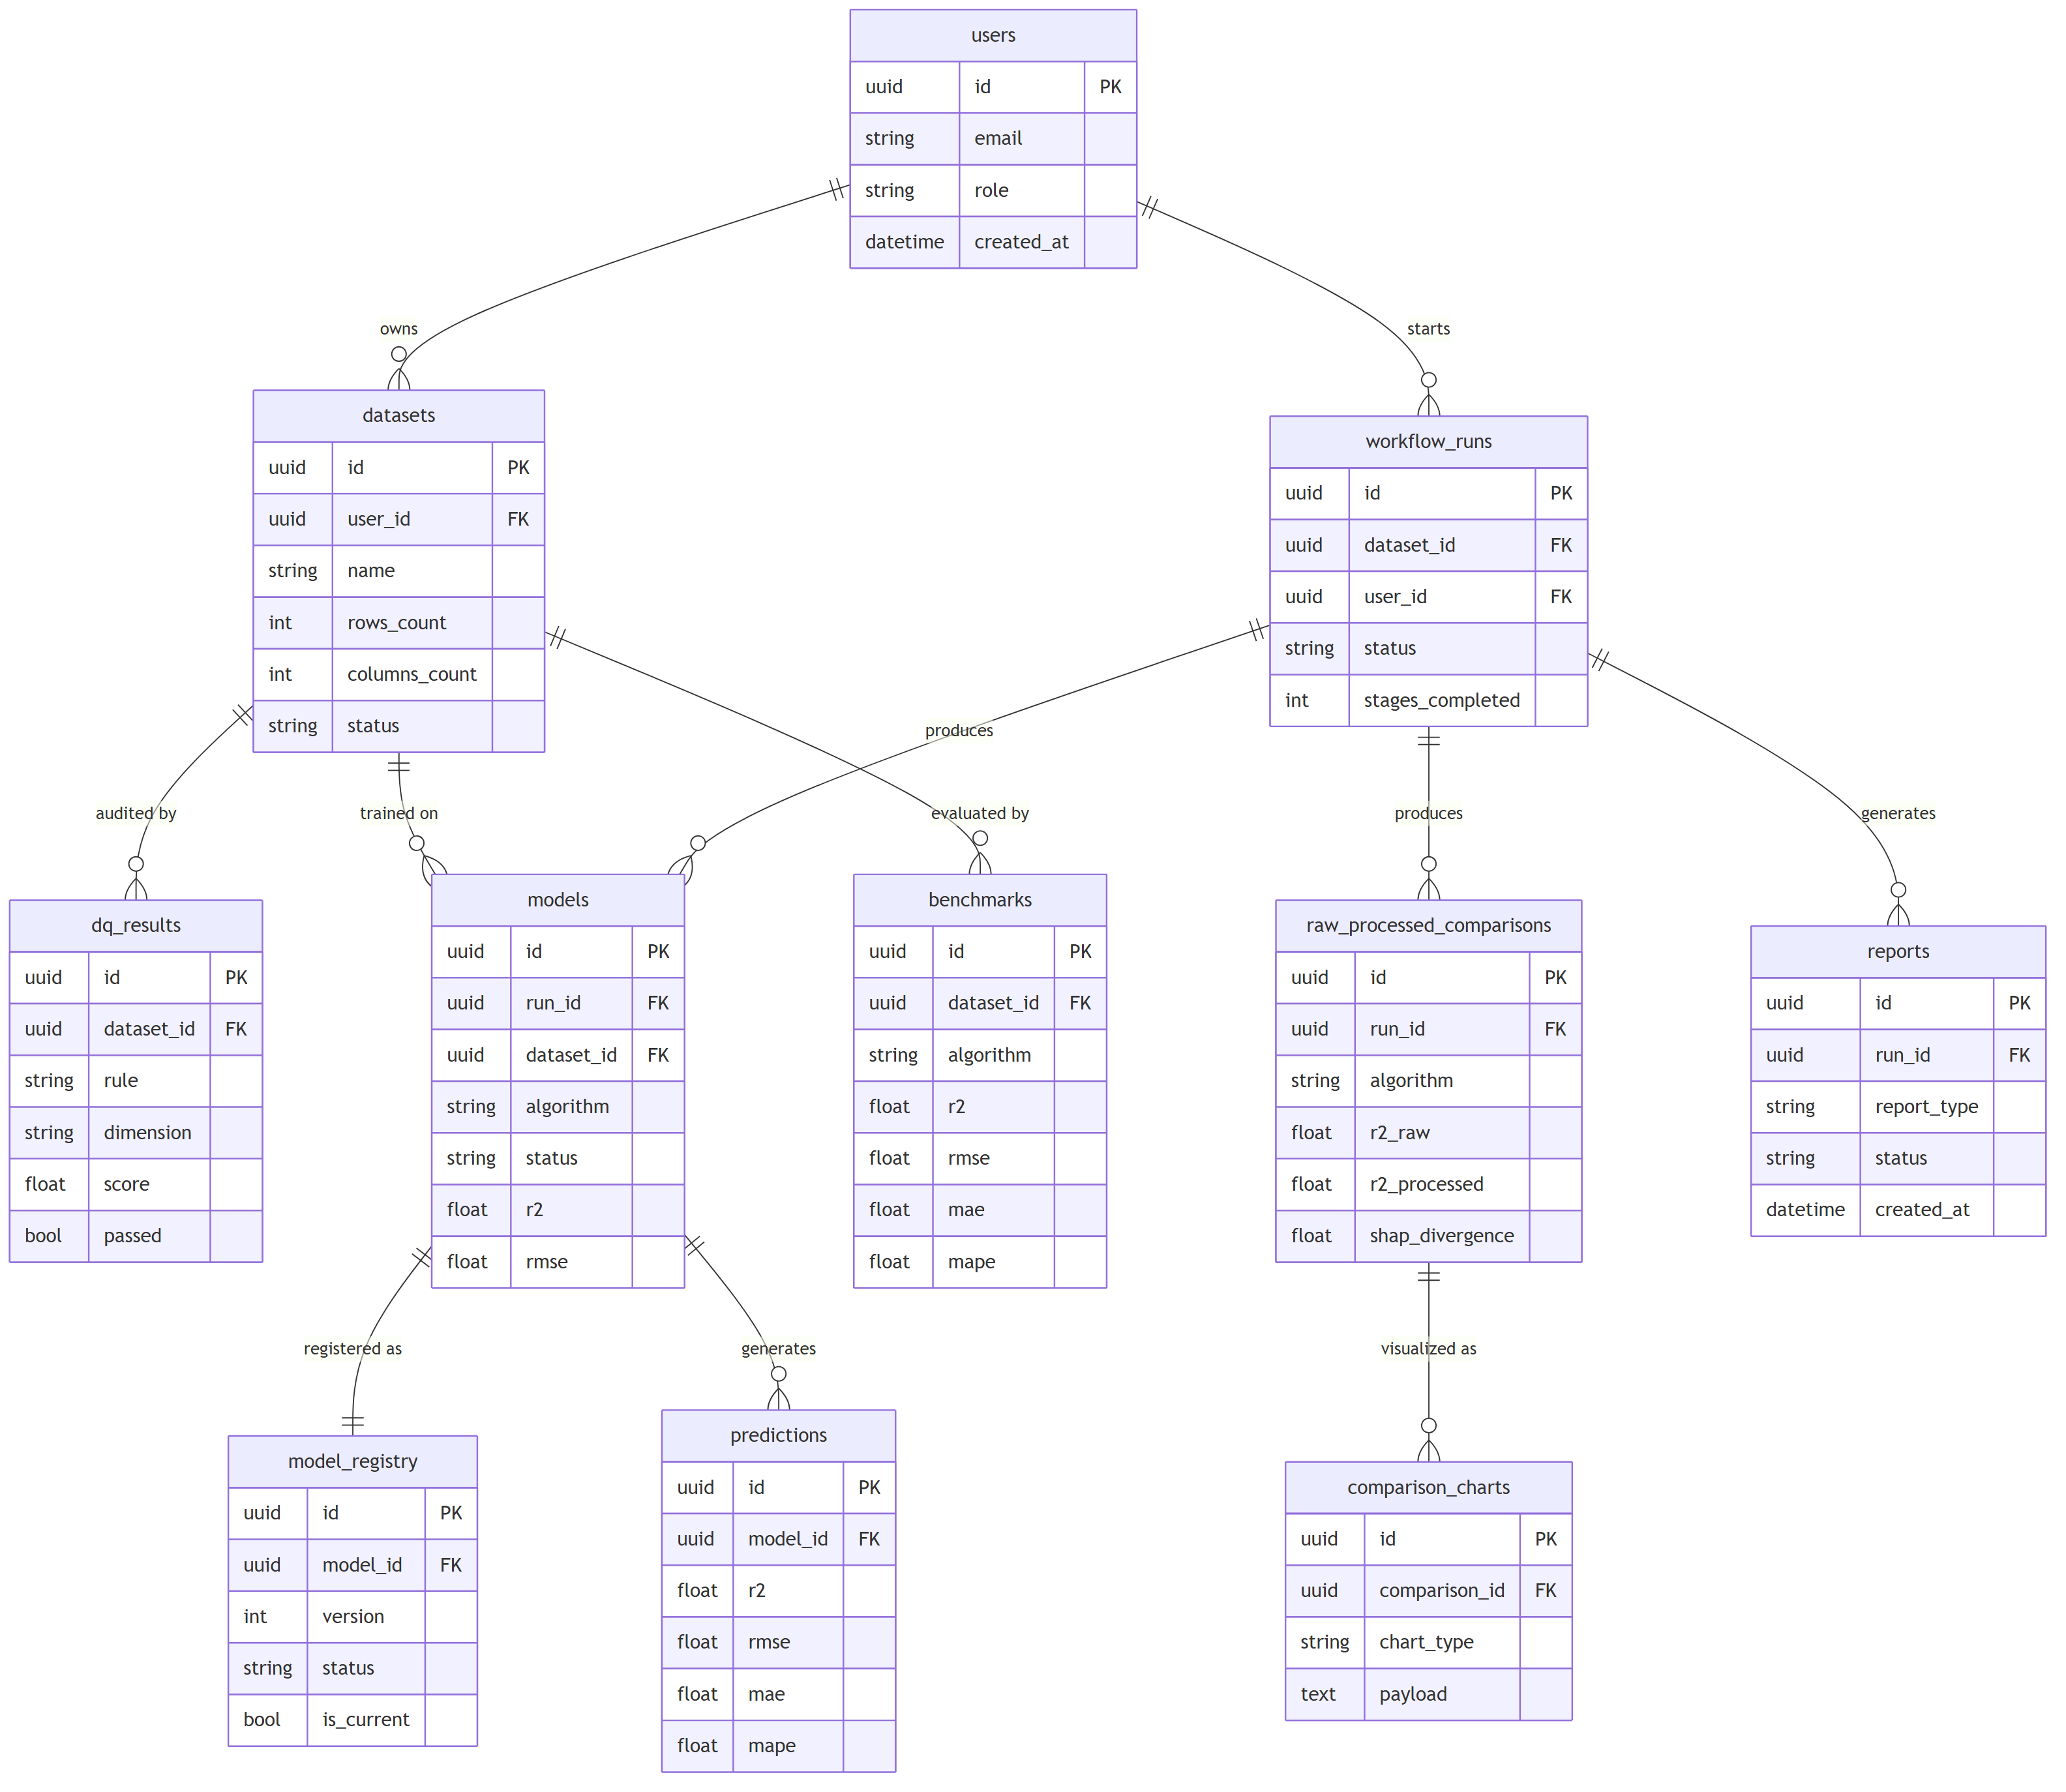
\includegraphics[width=\columnwidth]{er-diagram}
\caption{Core entity relationships (subset of the 21-table schema).}
\label{fig:er}
\end{figure}

\section{Data Quality Engine}\label{sec:dq}

\begin{figure}[!t]
\centering
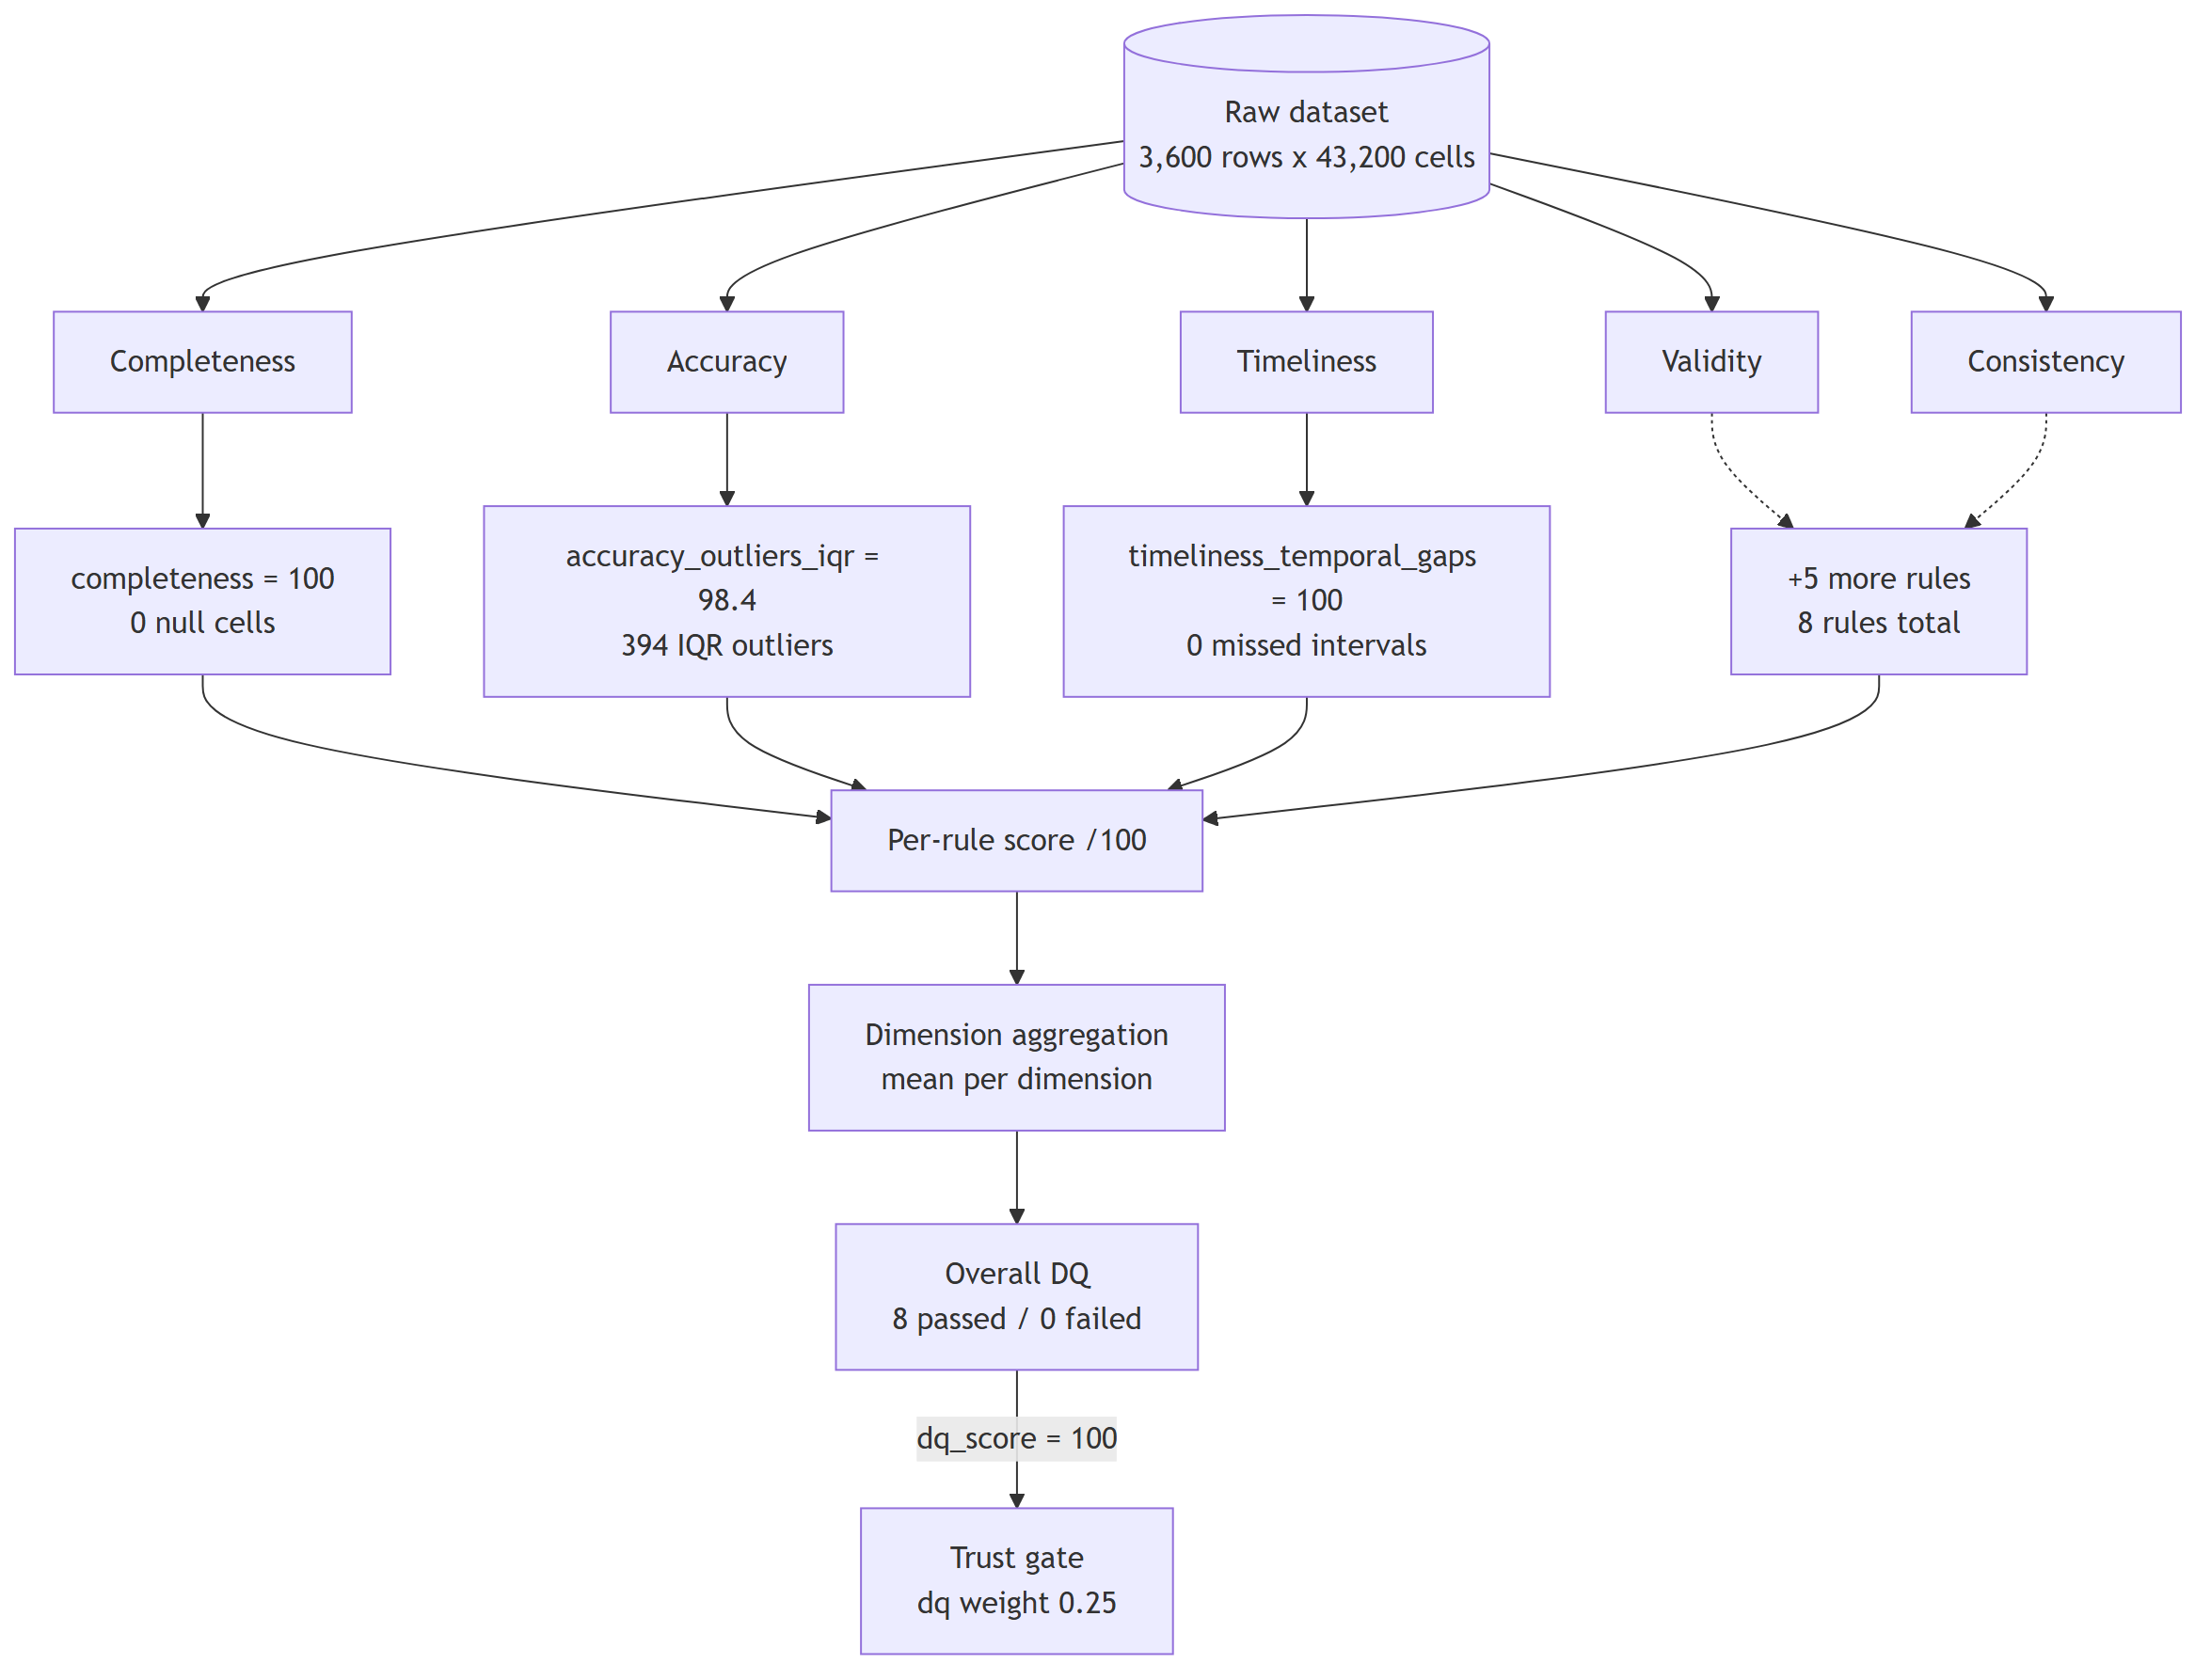
\includegraphics[width=\columnwidth]{data-quality-flow}
\caption{Data quality flow. Raw data is evaluated against 5 dimensions realized by 8 rules; per-rule scores on a 0--100 scale are aggregated by dimension and feed the trust gate with weight 0.25.}
\label{fig:dq}
\end{figure}

The DQ engine (Algorithms~\ref{alg:dq}--\ref{alg:outlier}, Fig.~\ref{fig:dq}) evaluates 8 rules grouped into the 5 dimensions of~\cite{wang:1996}. Each rule emits a score in $[0,100]$ and a \texttt{passed} flag using thresholds $s \ge 80$ for \texttt{info}/\texttt{warning} severity and $s \ge 70$ for \texttt{critical} severity. Results are persisted per run with structured detail payloads.

\begin{algorithm}[!t]
\caption{DataQualityAssessment}
\label{alg:dq}
\begin{algorithmic}[1]
\REQUIRE dataset $D$, target column $y$
\ENSURE per-rule scores $\{s_i\}$, dimension aggregates, overall
\STATE rules $\gets$ \{\textsc{Completeness}, \textsc{SemanticBounds}, \textsc{Duplicates}, \textsc{Monotonic}, \textsc{Identifiers}, \textsc{OutliersIQR}, \textsc{ZScore}, \textsc{TemporalGaps}\}
\FOR{each rule $r$ in rules}
  \STATE $s_r \gets$ \textsc{ScoreRule}($r$, $D$, $y$); persist $(r, s_r, \text{details})$
\ENDFOR
\STATE for each dimension $d$: $\bar{s}_d \gets \mathrm{mean}\{s_r : \mathrm{dim}(r)=d\}$
\STATE $\text{overall} \gets \big(\textstyle\sum_r s_r\big)\big/|\{d\}|$ \COMMENT{see caveat Sec.~\ref{sec:dq-score}}
\RETURN $\{s_r\}, \{\bar{s}_d\}, \text{overall}$
\end{algorithmic}
\end{algorithm}

\begin{algorithm}[!t]
\caption{CompletenessScore}
\label{alg:complete}
\begin{algorithmic}[1]
\REQUIRE dataset $D$ with $n$ rows, $m$ columns
\ENSURE score $s \in [0,100]$
\STATE $c \gets n \times m$; $n_{\text{null}} \gets$ count of null cells
\RETURN $100 \times (1 - n_{\text{null}}/c)$
\end{algorithmic}
\end{algorithm}

\begin{algorithm}[!t]
\caption{SemanticBoundsScore}
\label{alg:bounds}
\begin{algorithmic}[1]
\REQUIRE numeric columns $C$, bounds $[l_j,u_j]$
\ENSURE score $s \in [0,100]$
\STATE $t \gets 0$; $p \gets 0$
\FOR{each column $j \in C$ and each value $v$}
  \STATE $t \gets t+1$
  \IF{$l_j \le v \le u_j$}
    \STATE $p \gets p+1$
  \ENDIF
\ENDFOR
\RETURN $100 \times p/t$
\end{algorithmic}
\end{algorithm}

\begin{algorithm}[!t]
\caption{TemporalConsistencyScore}
\label{alg:temporal}
\begin{algorithmic}[1]
\REQUIRE timestamps $t_1,\ldots,t_n$
\ENSURE scores $(s_{\text{mono}}, s_{\text{gap}})$
\STATE $b \gets |\{i : t_{i+1} < t_i\}|$; \quad $s_{\text{mono}} \gets 100 \times (1 - b/n)$
\STATE $\delta_i \gets t_{i+1}-t_i$; \STATE $\tilde{\delta} \gets \mathrm{median}(\delta)$
\STATE $g \gets |\{i : \delta_i > 1.5\,\tilde{\delta}\}|$; \quad $s_{\text{gap}} \gets 100 \times (1 - g/n)$
\RETURN $s_{\text{mono}}, s_{\text{gap}}$
\end{algorithmic}
\end{algorithm}

\begin{algorithm}[!t]
\caption{OutlierScores (IQR + z-score)}
\label{alg:outlier}
\begin{algorithmic}[1]
\REQUIRE series $x$, target $y$, threshold $z_0=5$
\ENSURE scores $(s_{\text{iqr}}, s_z)$
\STATE $Q_1,Q_3 \gets \mathrm{quartiles}(x)$; \STATE $\mathrm{IQR} \gets Q_3-Q_1$
\STATE fences $\gets [Q_1-3\,\mathrm{IQR},\; Q_3+3\,\mathrm{IQR}]$ \COMMENT{3$\times$IQR}
\STATE $\rho \gets \mathrm{outlier\_rate}(x)$; \quad $s_{\text{iqr}} \gets \mathrm{clip}\big(100(1-\min(\rho,0.5)),\,50,\,100\big)$
\STATE $\mu,\sigma \gets \mathrm{mean,std}(y)$; \quad $e \gets |\{y_i : |y_i-\mu|/\sigma > z_0\}|$
\RETURN $s_{\text{iqr}},\; 100 \times (1 - e/|y|)$
\end{algorithmic}
\end{algorithm}

\subsection{Measured quality profile}\label{sec:dq-results}
Table~\ref{tab:dq} reports the evaluated dataset: 3{,}600 rows $\times$ 12 columns (43{,}200 cells), 5 assets, hourly sampling over 30 days (2{,}588{,}400\,s), target \texttt{energy\_kwh}. All 8 rules pass (6 \texttt{info}, 2 \texttt{warning}); scores range 96.7--100. Completeness is perfect (0 null cells), all 18{,}000 semantic-bound checks pass, and there are no duplicate rows. The two imperfect rules are informative rather than fatal: 120 non-monotonic timestamps (score 96.7) and 394 IQR outliers concentrated in \texttt{occupancy\_count} (315), \texttt{energy\_kwh} (41), and \texttt{power\_kw} (38), yielding 98.4 after the $\min(\rho,0.5)$ clamp.

\begin{table}[!t]
\caption{Data quality profile (per-rule scores are on a 0--100 scale)}
\label{tab:dq}
\centering
\begin{tabular}{@{}llr@{}}
\toprule
Rule & Dimension & Score \\
\midrule
completeness & completeness & 100 \\
validity\_semantic\_bounds & validity & 100 \\
consistency\_duplicates & consistency & 100 \\
consistency\_monotonic & consistency & 96.7 \\
validity\_identifiers & validity & 100 \\
accuracy\_outliers\_iqr & accuracy & 98.4 \\
accuracy\_zscore & accuracy & 99.9 \\
timeliness\_temporal\_gaps & timeliness & 100 \\
\midrule
passed / failed & --- & 8 / 0 \\
\bottomrule
\end{tabular}
\end{table}

\subsection{A scoring caveat}\label{sec:dq-score}
The aggregate \texttt{overall\_score} returned by the read endpoint is computed as $\big(\sum_r s_r\big)/|\{d\}|$, i.e.\ the sum of all rule scores divided by the number of distinct dimensions. For Table~\ref{tab:dq} this yields $795/5 = 159$, which is \emph{not} a percentage and is not bounded by 100; the write-path variant weights five dimension means by 0.25 each, so its weights sum to 1.25 (maximum 125). Both formulas are documented implementation artifacts. We therefore report per-rule scores and the trust gate's normalized DQ input (Section~\ref{sec:trust}) rather than the raw aggregate, and flag the aggregation as a defect to fix.

\section{Feature Engineering and Temporal Validation}\label{sec:feat}

\begin{algorithm}[!t]
\caption{DeriveTimeSeriesFeatures}
\label{alg:derive}
\begin{algorithmic}[1]
\REQUIRE frame with target series $y$ (hourly)
\ENSURE feature columns
\STATE \texttt{lag\_1h} $\gets \mathrm{shift}(y,1)$ \COMMENT{$y_{t-1}$}
\STATE \texttt{diff\_1h} $\gets \mathrm{diff}(y,1)$ \COMMENT{$y_t - y_{t-1}$}
\STATE \texttt{rolling\_24h} $\gets \mathrm{rolling}(y,24).\mathrm{mean}()$ \COMMENT{window includes $y_t$}
\STATE \texttt{load\_factor} $\gets y / \texttt{power\_kw}$; \quad \texttt{energy\_density} $\gets y / \texttt{occupancy}$
\RETURN derived columns
\end{algorithmic}
\end{algorithm}

\begin{algorithm}[!t]
\caption{TimeOrderedSplit}
\label{alg:split}
\begin{algorithmic}[1]
\REQUIRE $n$ rows
\ENSURE train index $I_{tr}$, test index $I_{te}$
\STATE $c \gets \lfloor 0.7\,n \rfloor$
\RETURN $I_{tr} \gets \{0..c-1\}$, \ $I_{te} \gets \{c..n-1\}$
\end{algorithmic}
\end{algorithm}

Feature engineering (Algorithm~\ref{alg:derive}) creates lag, difference, rolling, and ratio features from the target and covariates. The benchmark protocol (Algorithm~\ref{alg:split}) uses a single chronological 70/30 holdout---the same split for every algorithm---rather than shuffled $k$-fold, consistent with temporal evaluation practice~\cite{bergmeir:2012, hyndman:2021}.

\paragraph{Leakage case study.}
The current implementation derives features on the full frame \emph{before} splitting. Because \texttt{diff\_1h} $= y_t - y_{t-1}$ and \texttt{lag\_1h} $= y_{t-1}$, the target is reconstructible exactly: $y_t = \texttt{diff\_1h} + \texttt{lag\_1h}$. Two additional derived columns contain $y_t$ directly (\texttt{load\_factor}, \texttt{energy\_density}), and the 24-step rolling mean includes $y_t$ in its own window. A linear model can therefore solve the task algebraically. This is precisely why ridge regression attains $R^2=1.0000$ in Section~\ref{sec:bench} while tree models do not exploit the identity as cleanly. The corrective discipline is split-then-derive: hold out the test window first, then compute derived features using training-window statistics only. We report the artifact rather than hide it because it is the platform's own detection of a defect class that silent pipelines miss.

\section{Model Benchmarking}\label{sec:bench}

\begin{algorithm}[!t]
\caption{BenchmarkModels}
\label{alg:bench}
\begin{algorithmic}[1]
\REQUIRE feature matrix $X$, target $y$, algorithms $\mathcal{A}$
\ENSURE leaderboard
\STATE $I_{tr}, I_{te} \gets$ \textsc{TimeOrderedSplit}($n$) \COMMENT{Alg.~\ref{alg:split}}
\STATE $\hat{y}$ metrics $\gets$ \textsc{metrics\_dict}($y_{te}$, $\hat{y}$) $= (R^2, \mathrm{RMSE}, \mathrm{MAE}, \mathrm{MAPE}, EV)$
\FOR{each $a \in \mathcal{A}$}
  \STATE $m_a \gets \mathrm{fit}(a, X_{I_{tr}}, y_{I_{tr}})$; \quad $\hat{y} \gets m_a(X_{I_{te}})$
  \STATE record $(a, R^2, \mathrm{RMSE}, \mathrm{MAE}, \mathrm{MAPE}, EV)$
\ENDFOR
\RETURN sorted leaderboard
\end{algorithmic}
\end{algorithm}

\begin{table}[!t]
\caption{Benchmark leaderboard (chronological 70/30 holdout; GBM = gradient boosting)}
\label{tab:bench}
\centering
\begin{tabular}{@{}lrrrr@{}}
\toprule
Algorithm & $R^2$ & RMSE & MAE & MAPE \\
\midrule
xgboost & 0.9147 & 1.3740 & 0.1235 & 1.57 \\
random forest & 0.9162 & 1.3624 & 0.1191 & 1.44 \\
\textbf{gradient boosting} & \textbf{0.9175} & \textbf{1.3517} & \textbf{0.1120} & \textbf{1.32} \\
ridge$^{\dagger}$ & 1.0000 & 0.0048 & 0.0024 & 0.09 \\
\bottomrule
\multicolumn{5}{@{}l}{\footnotesize $^{\dagger}$target-leakage artifact; not a legitimate result (Sec.~\ref{sec:feat}).}
\end{tabular}
\end{table}

Table~\ref{tab:bench} reports the four-regressor benchmark. Among legitimate learners, gradient boosting ranks first on every metric ($R^2=0.9175$, RMSE 1.3517, MAE 0.1120, MAPE 1.32), followed by random forest and XGBoost~\cite{chen:2016} within 0.003 $R^2$ of each other; all three are tree ensembles in the tradition of~\cite{breiman:2001}, trained through scikit-learn~\cite{pedregosa:2011} with default hyperparameters. Ridge regression~\cite{hoerl:1970} attains $R^2=1.0000$ with RMSE 0.0048, which we attribute to the pre-split leakage of Section~\ref{sec:feat} rather than to superior fit; it is annotated accordingly in the table and excluded from model selection. The registry records the promoted gradient-boosting candidate with 17 engineered features and 2{,}091 training rows.

\section{Explainability and the Trust Gate}\label{sec:trust}

\begin{algorithm}[!t]
\caption{ExplanationStabilityIndex}
\label{alg:stab}
\begin{algorithmic}[1]
\REQUIRE model $f$, matrix $X$ ($n \ge 40$ rows)
\ENSURE stability index $\in [0,100]$
\STATE partition rows randomly into halves $X_a, X_b$
\STATE $A \gets \mathrm{mean}|{\rm SHAP}|(f, X_a)$; \quad $B \gets \mathrm{mean}|{\rm SHAP}|(f, X_b)$
\STATE $\rho \gets \mathrm{Spearman}(\mathrm{argsort}(A), \mathrm{argsort}(B))$
\RETURN $100 \times \max(0, \rho)$ \COMMENT{default 70 if $n<40$}
\end{algorithmic}
\end{algorithm}

\begin{algorithm}[!t]
\caption{TrustGate}
\label{alg:gate}
\begin{algorithmic}[1]
\REQUIRE factors $c_{\text{pred}}, s_{\text{dq}}, r_{\text{model}}, s_{\text{shap}} \in [0,100]$
\ENSURE trust score, verdict
\STATE $T \gets 0.40\,c_{\text{pred}} + 0.25\,s_{\text{dq}} + 0.20\,r_{\text{model}} + 0.15\,s_{\text{shap}}$
\STATE verdict $\gets$ \texttt{high\_trust} if $T \ge 90$, \texttt{medium} if $T \ge 70$, else \texttt{low}
\RETURN $T$, verdict
\end{algorithmic}
\end{algorithm}

Global explanations use SHAP TreeExplainers~\cite{lundberg:2017} to rank features by mean absolute attribution. Explanation quality is not assumed: Algorithm~\ref{alg:stab} measures whether feature \emph{rankings} reproduced on two random half-samples agree (Spearman correlation), stored as the stability index. We distinguish this from a second, mislabeled metric present in the comparison module---a Pearson correlation between the argsorted magnitude vector and the identity ramp, clamped at zero---which measures column-order alignment rather than stability and is non-reproducible across calls because it resamples without a seed. We report the genuine index and flag the mislabeled one for correction.

The confidence gate (Algorithm~\ref{alg:gate}) fuses four evidence factors with fixed weights 0.40 (prediction confidence), 0.25 (DQ score), 0.20 (model relevance), and 0.15 (explanation stability). On the evaluated dataset the factors are $100$, $100$, $91.5$, and $75$, giving
\[
T = 0.40(100) + 0.25(100) + 0.20(91.5) + 0.15(75) = 94.5,
\]
a \texttt{high\_trust} verdict. The gate is an auditable composite, not a probabilistic calibrator in the sense of~\cite{guo:2017}; its purpose is to make deployment decisions traceable to named evidence.

\section{Raw vs.\ Processed: An Honest Null Result}\label{sec:rawproc}

\begin{algorithm}[!t]
\caption{RawVsProcessedComparison}
\label{alg:cmp}
\begin{algorithmic}[1]
\REQUIRE run $r$, algorithm $a$, dataset $D$
\ENSURE metrics, deltas, conclusion
\STATE load raw frame $D_{raw}$ and cleaned frame $D_{proc}$; derive features on each
\STATE $I_{tr}, I_{te} \gets$ \textsc{TimeOrderedSplit}; \quad restrict both to common feature columns
\STATE fit identical model $a$ on $(D_{raw})$ and on $(D_{proc})$; evaluate on their test windows
\STATE $\Delta R^2 \gets R^2_{proc} - R^2_{raw}$; \quad $\Delta_{\text{stab}} \gets s_{raw} - s_{proc}$
\STATE divergence $\gets |\Delta_{\text{stab}}| + |\Delta R^2|$; \quad persist comparison + charts
\RETURN metrics, deltas, conclusion
\end{algorithmic}
\end{algorithm}

\begin{table}[!t]
\caption{Raw vs.\ processed comparison (XGBoost, 17 features per side)}
\label{tab:rawproc}
\centering
\begin{tabular}{@{}llrrrr@{}}
\toprule
Run & Side & $R^2$ & RMSE & MAE & $s_{\text{shap}}$ \\
\midrule
\multirow{2}{*}{A} & raw & 0.9153 & 1.3692 & 0.121 & 11.0 \\
 & proc. & 0.9153 & 1.3692 & 0.121 & 5.9 \\
\midrule
\multirow{2}{*}{B} & raw & 0.9153 & 1.3692 & 0.121 & 9.1 \\
 & proc. & 0.9153 & 1.3692 & 0.121 & 0.0 \\
\bottomrule
\end{tabular}
\end{table}

Table~\ref{tab:rawproc} reports two comparison runs in which identical XGBoost models were trained on raw versus cleaned data under the same chronological split. Predictive metrics are \emph{identical} on both sides ($R^2=0.9153$, RMSE 1.3692, MAE 0.121, MAPE 1.58), so $\Delta R^2 = 0.000$ and all error deltas are zero; only the (mislabeled) column-order index differs (raw 11.0/9.1 vs.\ processed 5.9/0.0), producing divergences of 5.1 and 9.1. The platform's own generated conclusion reads: ``Raw data matched or beat cleaned data here---possible over-cleaning or already-high quality input.''

This null result is the expected outcome for an input that already passes every DQ rule (Table~\ref{tab:dq}): cleaning cannot improve accuracy when there is little left to fix, and aggressive transforms risk discarding signal. We regard the finding as supporting, not undermining, the data-quality-first thesis---the value of the comparison stage is to \emph{measure} whether cleaning helped on \emph{this} dataset rather than assume it universally~\cite{wang:1996}.

\section{Workflow, Interface, and Reproducibility}\label{sec:ui}

\begin{figure*}[!t]
\centering
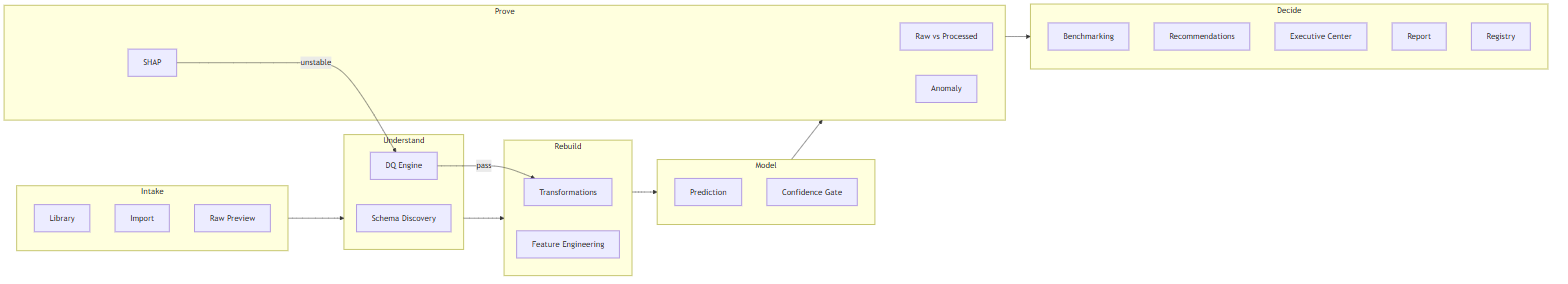
\includegraphics[width=\textwidth]{workflow-pipeline}
\caption{The 17-stage EcoMind-AI workflow grouped into six milestones (Intake, Understand, Rebuild, Model, Prove, Decide). The confidence gate branches on the trust verdict; stages may re-clean data and re-enter the loop.}
\label{fig:pipeline}
\end{figure*}

The workflow (Fig.~\ref{fig:pipeline}) is driven from a single-page client. Stage execution is explicit---either manual (operator clicks \emph{Run}) or automatic (SSE-driven \texttt{AutoNext})---and every transition is persisted, so the history view can reconstruct stage timings. The benchmark leaderboard supports CSV export, reports render to PDF, and a progress ring resumes a run where it left off.

\begin{figure*}[!t]
\centering
\begin{minipage}[t]{0.49\textwidth}
\centering

\includegraphics[width=\linewidth]{dashboard}
\end{minipage}\hfill
\begin{minipage}[t]{0.49\textwidth}
\centering
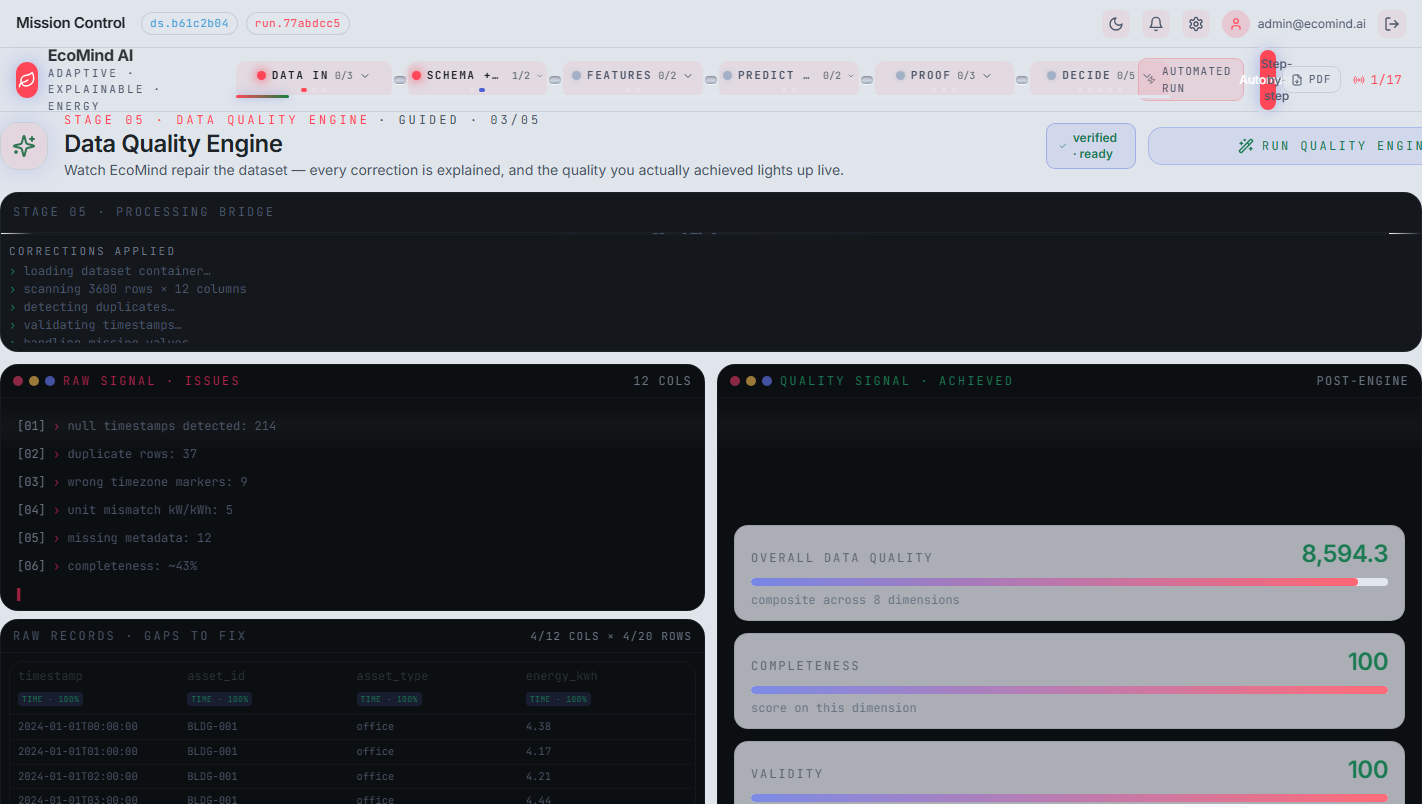
\includegraphics[width=\linewidth]{dqengine}
\end{minipage}
\caption{Production UI (captured from the live deployment). Left: the Mission Control dashboard with workflow progress, business impact, and executive narrative. Right: the data quality engine screen showing rule-level scores. Known visual inconsistency: the DQ screen uses dark terminal panels inside the otherwise light glass theme.}
\label{fig:ui}
\end{figure*}

Reproducibility constraints are deliberate: the system runs fully offline (no external model registry, no cloud calls at run time), all artifacts live in a single SQLite file, and the benchmark split is deterministic given the input file. Current measured test status: 7 backend tests (pytest), 22 frontend tests (vitest), and a clean TypeScript + Vite build.

\section{Limitations and Discussion}\label{sec:limits}
\begin{itemize}
\item \textbf{Dataset scale.} Headline results come from a 3{,}600-row hourly, 5-asset corpus. Absolute error values (RMSE $\approx 1.35$) are dataset-specific; the protocol, not the numbers, is the transferable contribution. Larger public corpora such as BDG2~\cite{miller:2020} are the natural next substrate.
\item \textbf{Deterministic-split caveat.} All eight trained models record identical predictive metrics ($R^2=0.9153$), consistent with a single deterministic split reused across runs; we report this as observed rather than as eight independent confirmations.
\item \textbf{Known defects.} (i) DQ aggregate scores are unbounded/mis-weighted (Sec.~\ref{sec:dq-score}); (ii) the comparison module's \texttt{shap\_stability} field is a mislabeled column-order statistic, non-reproducible due to unseeded sampling; (iii) feature derivation precedes the split (Sec.~\ref{sec:feat}); (iv) workflow runs remain \texttt{running} until explicitly advanced, so \texttt{running} in the history list denotes mid-flight state, not failure; (v) the seed loader injects a \texttt{completed} run whose stage bookkeeping is integer-based and inconsistent with the key-based engine. Each is documented with a fix path in the project knowledge base.
\item \textbf{Gate semantics.} The trust gate is a weighted composite of heuristics, not a calibrated probability; weights are fixed engineering choices, not learned.
\item \textbf{Visual consistency.} The DQ screen's dark panels inside the light theme (Fig.~\ref{fig:ui}) are a known UI inconsistency under cleanup.
\end{itemize}

\section{Conclusion}

EcoMind-AI demonstrates that data quality assessment, leakage-aware benchmarking, explanation stability, and deployment gating can be unified into one offline, auditable pipeline whose numbers are traceable end to end. On our reference dataset the platform reports all DQ rules passing (96.7--100 per rule), ranks gradient boosting best among legitimate models ($R^2=0.9175$), detects a real target-leakage artifact ($R^2=1.0000$ for ridge), and fuses evidence into a 94.5/100 trust verdict---while honestly reporting that raw-versus-processed cleaning changed nothing ($\Delta R^2=0$) on already-clean data. Future work includes split-then-derive enforcement, corrected DQ aggregation, a seeded stability metric, evaluation on BDG2-scale corpora, and learned gate weights validated against downstream forecast outcomes.

\begin{thebibliography}{14}
\bibitem{amasyali:2018}
K.~Amasyali and N.~M. El-Gohary, ``A review of data-driven building energy consumption prediction studies,'' \emph{Renewable and Sustainable Energy Reviews}, vol.~81, pp. 1192--1205, 2018.

\bibitem{bergmeir:2012}
C.~Bergmeir and J.~M. Ben\'{i}tez, ``On the use of cross-validation for time series predictor evaluation,'' \emph{Information Sciences}, vol. 191, pp. 192--213, 2012.

\bibitem{breiman:2001}
L.~Breiman, ``Random forests,'' \emph{Machine Learning}, vol.~45, no.~1, pp. 5--32, 2001.

\bibitem{chen:2016}
T.~Chen and C.~Guestrin, ``XGBoost: A scalable tree boosting system,'' in \emph{Proc. 22nd ACM SIGKDD Int. Conf. Knowledge Discovery and Data Mining (KDD)}, 2016, pp. 785--794.

\bibitem{guo:2017}
C.~Guo, G.~Pleiss, Y.~Sun, and K.~Q. Weinberger, ``On calibration of modern neural networks,'' in \emph{Proc. 34th Int. Conf. Machine Learning (ICML)}, vol.~70, 2017, pp. 1321--1330.

\bibitem{hoerl:1970}
A.~E. Hoerl and R.~W. Kennard, ``Ridge regression: Biased estimation for nonorthogonal problems,'' \emph{Technometrics}, vol.~12, no.~1, pp. 55--67, 1970.

\bibitem{hyndman:2021}
R.~J. Hyndman and G.~Athanasopoulos, \emph{Forecasting: Principles and Practice}, 3rd~ed. Melbourne, Australia: OTexts, 2021.

\bibitem{lundberg:2017}
S.~M. Lundberg and S.-I. Lee, ``A unified approach to interpreting model predictions,'' in \emph{Advances in Neural Information Processing Systems 30 (NIPS)}, 2017, pp. 4768--4777.

\bibitem{miller:2020}
C.~Miller \emph{et al.}, ``The Building Data Genome Project 2, energy meter data from the ASHRAE Great Energy Predictor III Competition,'' \emph{Scientific Data}, vol.~7, no.~1, p. 368, 2020.

\bibitem{miller:2020gep}
C.~Miller \emph{et al.}, ``The ASHRAE Great Energy Predictor III Competition: Overview and results,'' \emph{Science and Technology for the Built Environment}, vol.~26, no.~10, pp. 1427--1447, 2020.

\bibitem{pedregosa:2011}
F.~Pedregosa \emph{et al.}, ``Scikit-learn: Machine learning in Python,'' \emph{Journal of Machine Learning Research}, vol.~12, pp. 2825--2830, 2011.

\bibitem{tukey:1977}
J.~W. Tukey, \emph{Exploratory Data Analysis}. Reading, MA, USA: Addison-Wesley, 1977.

\bibitem{wang:1996}
R.~Y. Wang and D.~M. Strong, ``Beyond accuracy: What data quality means to data consumers,'' \emph{Journal of Management Information Systems}, vol.~12, no.~4, pp. 5--33, 1996.

\bibitem{christ:2018}
M.~Christ, N.~Braun, J.~Neuffer, and A.~W. Kempa-Liehr, ``Time series feature extraction on basis of scalable hypothesis tests (tsfresh---a Python package),'' \emph{Neurocomputing}, vol. 307, pp. 72--77, 2018.
\end{thebibliography}

\end{document}
